% Created 2024-09-02 Mon 19:41
% Intended LaTeX compiler: pdflatex
\documentclass[letterpaper, 12pt]{article}
\usepackage[utf8]{inputenc}
\usepackage[T1]{fontenc}
\usepackage{graphicx}
\usepackage{longtable}
\usepackage{wrapfig}
\usepackage{rotating}
\usepackage[normalem]{ulem}
\usepackage{amsmath}
\usepackage{amssymb}
\usepackage{capt-of}
\usepackage{hyperref}
\usepackage{minted}
\usepackage{xcolor}
\usepackage{hyperref}
\usepackage{tocloft}
\usepackage{minted}
\usemintedstyle{manni}
\usepackage{pdfpages}
\usepackage{fancyhdr}
\usepackage{graphicx}
\usepackage[top=1.4in, left=0.5in, right=0.5in, bottom=0.8in]{geometry}
\usepackage[T1]{fontenc}
\usepackage{helvet}
\pagestyle{fancy}
\renewcommand{\headrulewidth}{0pt}
\renewcommand{\footrulewidth}{0pt}
\setlength{\parindent}{0em}
\setlength{\parskip}{1em}
\usepackage{hyperref}
\usepackage {color}
\usepackage {tabularray}
\usepackage{xcolor}
\hypersetup{
colorlinks=true,
linkcolor=blue,
filecolor=magenta,
urlcolor=cyan,
citecolor=green,
pdfborder={0 0 0}
}
\usepackage[most]{tcolorbox}
\author{Hilduara Abreu}
\date{\today}
\title{PS192 | Welcome Letters Academic Year 2024-25\\\medskip
\large English Version}
\hypersetup{
 pdfauthor={Hilduara Abreu},
 pdftitle={PS192 | Welcome Letters Academic Year 2024-25},
 pdfkeywords={},
 pdfsubject={},
 pdfcreator={Emacs 29.4 (Org mode 9.6.15)}, 
 pdflang={English}}
\begin{document}

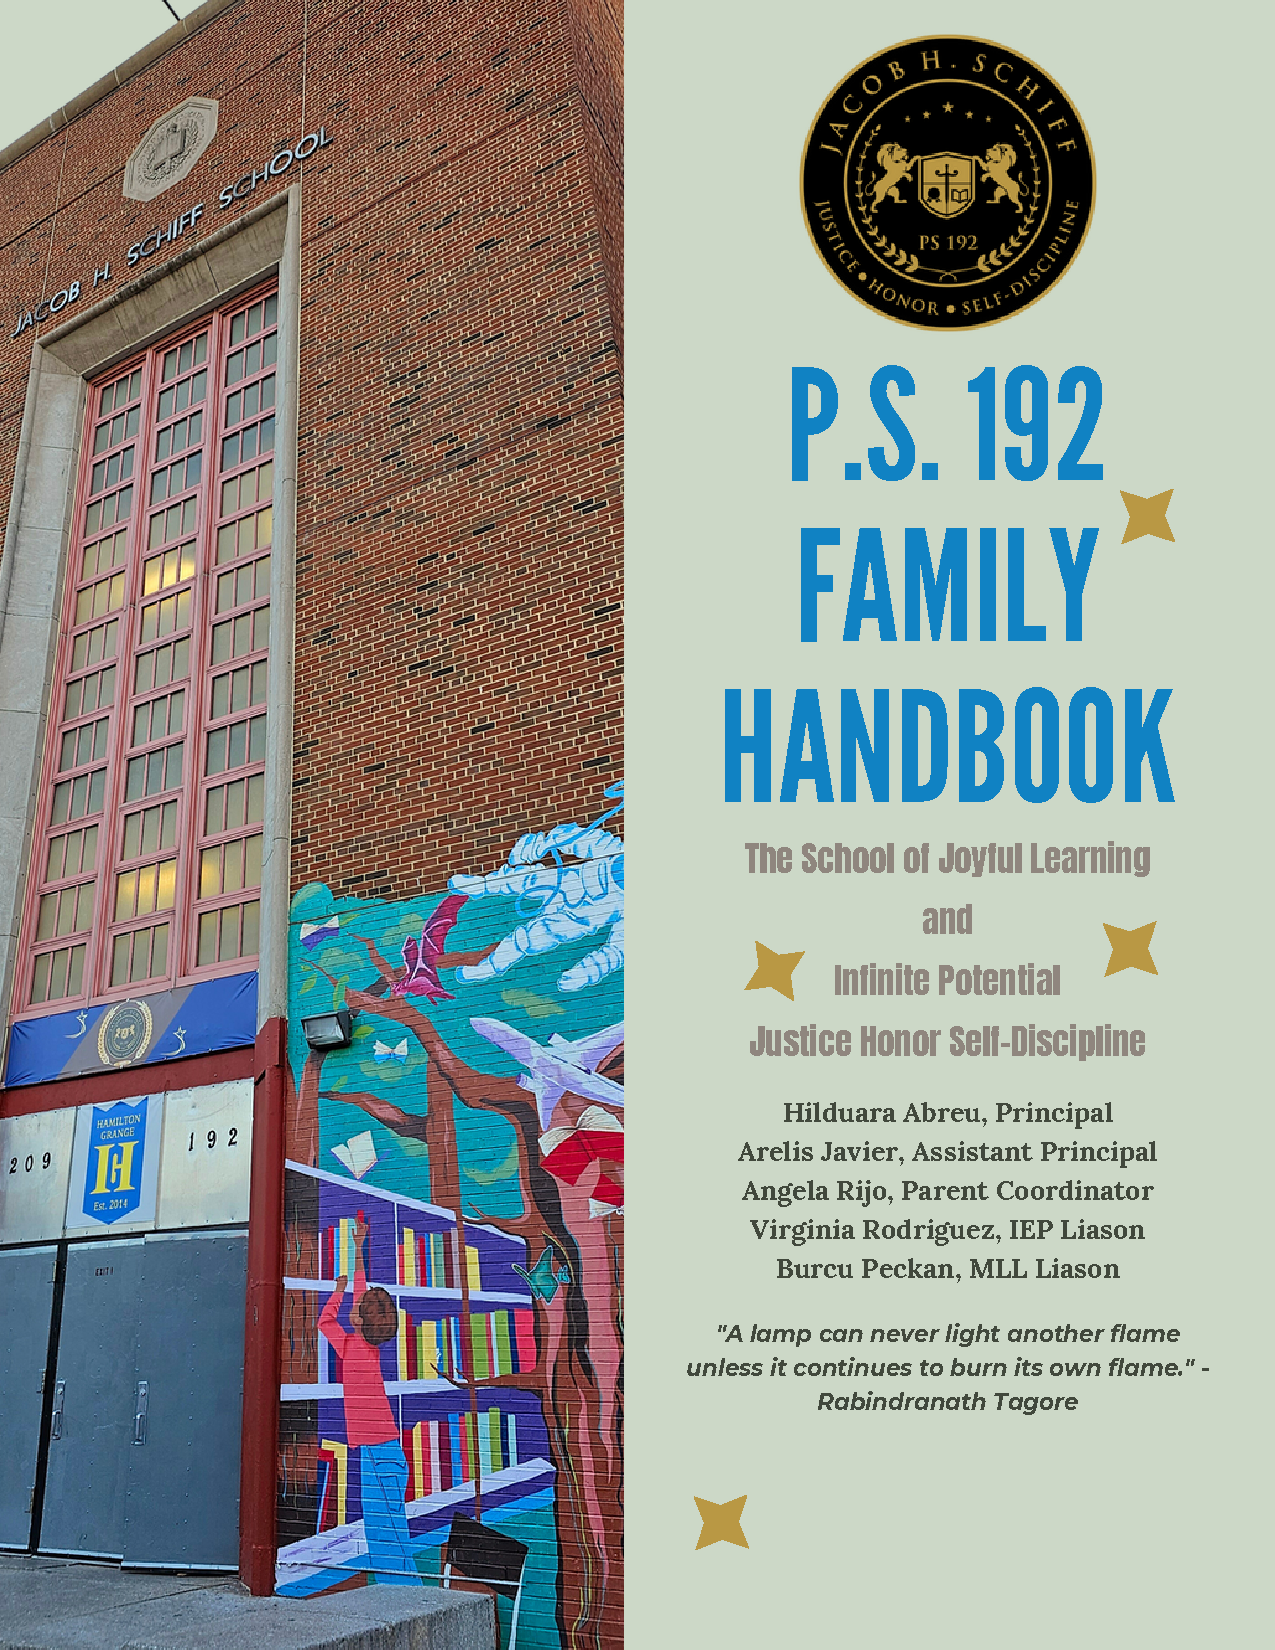
\includepdf[pages=1,fitpaper]{/home/rob/ps192_welcome_letters/2024/Welcome_Letters-En/pdf.pdf}

\fancyfoot[C]{\setlength{\unitlength}{1in}\begin{picture}(5,0)\put(-1.8,-0.5){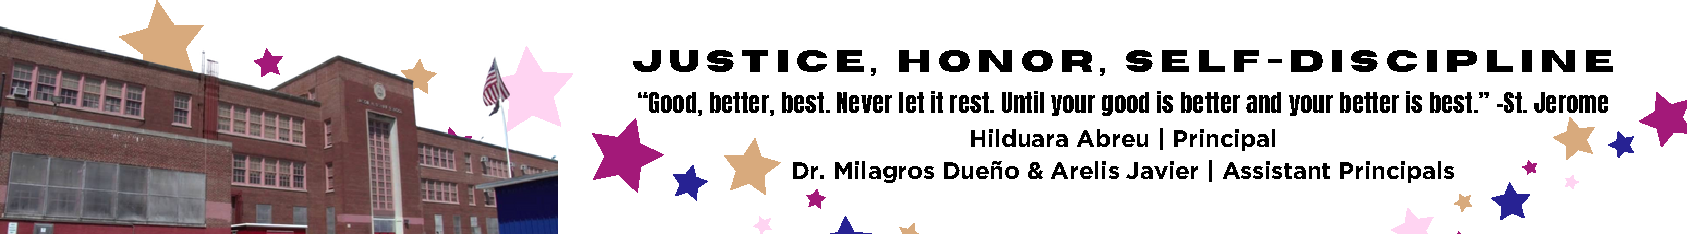
\includegraphics[width=8.8in,height=1.3in]{logo-1}}\end{picture}}
\fancyhead[C]{\setlength{\unitlength}{1in}\begin{picture}(5,0)\put(-1.9,-0.5){
\includegraphics[width=8.9in,height=1.3in]{logo-2}}\end{picture}}
\fancyhead[R]{\thepage}
\pagenumbering{gobble}

\begin{document}
\newpage
\vspace*{-0.5cm}

\section*{Table of Contents}
\label{sec:orgf9c70d2}
\begin{itemize}
\item \hyperref[sec:orgd9f8d08]{Introduction}
\item \hyperref[sec:org77a89b8]{Bell Schedule}
\item \hyperref[sec:orgcca2c0e]{Uniform Policy}
\item \hyperref[sec:org6922eaa]{Use of Electronic Devices}
\item \hyperref[sec:org5043dc4]{Violations and Disciplinary Actions}
\item \hyperref[sec:orgf2c6c95]{Welcome Letter 3-K and Pre-K}
\item \hyperref[sec:org8bf15a2]{Welcome Letter Grades K-5}
\item \hyperref[sec:org22babf9]{Promotional Criteria and Grading Policy}
\item \hyperref[sec:orgfbabc58]{Visitor and Safety Guidelines Procedures}
\item \hyperref[sec:org0878644]{Missing Student Protocol}
\end{itemize}

\newpage
\vspace*{-0.5cm}

\tcbuselibrary{}
\newtcolorbox{bluebox}[1][]{
  colback=blue!5!white,
  colframe=blue!75!black,
  fonttitle=\bfseries,
  coltitle=black,
  enhanced,
  attach boxed title to top center={yshift=-2mm},
  title=#1,
  boxed title style={colback=blue!50!white}
}
\newtcolorbox{greenbox}[1][]{
  colback=green!5!white,
  colframe=green!75!black,
  fonttitle=\bfseries,
  coltitle=black,
  enhanced,
  attach boxed title to top center={yshift=-2mm},
  title=#1,
  boxed title style={colback=green!50!white}
}
\newtcolorbox{redbox}[1][]{
  colback=red!5!white,
  colframe=red!75!black,
  fonttitle=\bfseries,
  coltitle=black,
  enhanced,
  attach boxed title to top center={yshift=-2mm},
  title=#1,
  boxed title style={colback=red!50!white}
}

\section*{Introduction}
\label{sec:orgd9f8d08}
Dear Parent or Guardian,

Welcome to PS 192! We are committed to providing a safe and nurturing environment where every student can thrive academically, socially, and emotionally. As we embark on another exciting school year, it is essential for all members of our school community to stay informed about our policies, rules, events, and core values. These guidelines help us create a positive and productive learning atmosphere for our students.

\begin{quote}
"Education is the journey where Justice, Honor, and Self-Discipline guide us to
unlock our fullest potential. At PS 192, we believe in cultivating these core
values to inspire greatness in every student, parent, and teacher, setting the
foundation for a brighter future. Together, let's embark on this new academic
year with a shared commitment to excellence and a passion for lifelong
learning."   -- Hilduara Abreu
\end{quote}

At PS 192, we believe in the power of education to transform lives. Our dedicated staff works tirelessly to offer the highest quality education, empowering our students to become the next generation of thinkers and leaders who will make a positive impact on our city and beyond. Your partnership and support are crucial in this journey, and we thank you for being an integral part of our community.

Together, we can ensure that PS 192 continues to be a place where every child feels valued and inspired to reach their full potential. We look forward to a successful and enriching school year with your continued involvement and cooperation.

With Justice, Honor, and Self-Discipline,


\includegraphics[width=0.2\textwidth]{hil_signature}

\textbf{Hilduara Abreu, Principal}

\textbf{The school of Joyful Learning!}

\href{www.ps192.org}{www.ps192.org}
\pagebreak
\vspace*{-0.5cm}

\subsection*{Bell Schedule}
\label{sec:org77a89b8}
Dear Parent or Guardian,

A bell schedule specifies the start time and duration of one or more instructional periods on each day of a day pattern. A consistent daily schedule and step-by-step routines give children a predictable day. A Bell Schedule helps children:
\begin{itemize}
\item Feel in control of their environment
\item Feel safe, secure, and comfortable
\item Know what is happening now and what comes next
\item Know how to do an activity or task
\item Engage in learning
\end{itemize}

Just like adults, children feel more confident and secure when their daily activities are predictable and familiar.

\begin{bluebox}[PS 192 | Bell Schedule]
\begin{table}[H]
\centering
\begin{tblr}{
  colspec={|X|X|X|X|},
  row{1}={font=\bfseries\color{MacaroniandCheese},c},
  hlines,
  vlines,
  hline{1,10} = {-}{0.08em},
}
\textbf{Period} & \textbf{Start Time} & \textbf{End Time} & \textbf{Length} \\
1               & 08:00 AM            & 08:45 AM          & 45 minutes      \\
2               & 08:45 AM            & 09:30 AM          & 45 minutes      \\
3               & 09:30 AM            & 10:15 AM          & 45 minutes      \\
4               & 10:15 AM            & 11:05 AM          & 50 minutes      \\
5               & 11:05 AM            & 11:55 AM          & 50 minutes      \\
6               & 11:55 AM            & 12:40 PM          & 45 minutes      \\
7               & 12:40 PM            & 01:30 PM          & 50 minutes      \\
8               & 01:30 PM            & 02:15 PM          & 45 minutes
\end{tblr}
\end{table}
\end{bluebox}

\pagebreak
\vspace*{0.5cm}

With Justice, Honor, and Self-Discipline,


\includegraphics[width=0.2\textwidth]{hil_signature}

\textbf{Hilduara Abreu, Principal}

\textbf{The school of Joyful Learning!}

\href{www.ps192.org}{www.ps192.org}

\pagebreak
\vspace*{-0.5cm}

\subsection*{Uniform Policy}
\label{sec:orgcca2c0e}
Dear Parent or Guardian,

The uniform policy will be enforced during school hours and at all school-related events and activities, such as field trips and special assemblies.
\begin{enumerate}
\item \textbf{Burgundy Shirt}: All students are required to wear a burgundy-colored shirt as the upper part of their uniform.
\item \textbf{Navy Pants}: Navy blue pants or trousers are to be worn as the lower part of the uniform.
\end{enumerate}

\textbf{\textbf{Benefits of the Uniform Policy}}

Uniforms serve as a unifying element within our school community and offer several significant advantages:

\begin{enumerate}
\item \textbf{Promoting Equality}: Uniforms eliminate socioeconomic disparities among students, ensuring that everyone is dressed the same way, regardless of their family’s financial circumstances.
\item \textbf{Enhancing Focus}: Wearing uniforms reduces distractions related to fashion and peer pressure, allowing students to concentrate on their studies and personal growth.
\item \textbf{Fostering School Pride}: A uniform instills a sense of pride and belonging among students, helping them identify with and appreciate their school community.
\item \textbf{Improving Safety}: Uniforms make it easier to identify intruders on school premises, enhancing overall security.
\item \textbf{Preparing for Future Success}: Encouraging a dress code similar to
professional attire helps prepare students for future careers where a
professional appearance is important.
\end{enumerate}

\textbf{\textbf{Dress Down Days}}

We understand that personal expression is important, and therefore, "Dress Down
Days" will be occasionally scheduled throughout the school year, allowing
students to express their individuality through clothing choices. We kindly
request your cooperation and support in ensuring that your child arrives at
school dressed in accordance with our uniform policy. We believe that this will
contribute to a more positive and productive learning environment for all
students.

\pagebreak
\vspace*{-0.5cm}

\textbf{Contact Information}

Should you have any questions or concerns regarding the uniform policy, please feel free to reach out to our Parent Coordinator, Ms. Angela Rijo, via the following channels:
\begin{itemize}
\item Website: \url{https://www.ps192.org/angela}
\item Whatsapp Group
\item ClassDojo
\item Phone: (212) 775-9560
\item In person during office hours: 9:00 AM - 3:00 PM
\end{itemize}

We are here to assist and support you.

\textbf{\textbf{Closing}}

Thank you for your partnership in nurturing a strong and vibrant learning community at P.S. 192. We look forward to a successful and enriching academic year ahead.

With Justice, Honor, and Self-Discipline,


\includegraphics[width=0.2\textwidth]{hil_signature}

\textbf{Hilduara Abreu, Principal}

\textbf{The School of Joyful Learning!}

\href{https://www.ps192.org}{www.ps192.org}
\pagebreak
\vspace*{-0.5cm}

\subsection*{Use of Electronic Devices}
\label{sec:org6922eaa}
Dear Parent or Guardian,

\begin{redbox}[PS 192 | Policy]
Prohibited Devices
Although not recommended, students are allowed to bring the following electronic items to school:
\begin{itemize}
\item Cell phones
\item Portable music and entertainment systems (e.g., iPods, MP3 players)
\end{itemize}
\textit{The student and/or parent is responsible for the safety and security of these devices. The school does not provide facilities to charge devices.}
\vspace*{3mm}

Important Key Points:
\begin{itemize}
\item Before 8:00 AM or after 3:35 PM in any location within the school where it does not disrupt educational activities.
\item Be turned on or used during instructional time, except for educational purposes with the teacher's approval.
\item Be turned on or used during quizzes, tests, or exams unless explicitly authorized or as part of an Individualized Education Program (IEP) or Section 504 Accommodation Plan.
\item Be in the possession of students during the school's bell schedule.
\item Be turned on or used during fire drills or other emergency preparedness exercises.
\item Be used in bathrooms.
\item Be used during lunch in the cafeteria or schoolyard.
\item Be used between classes in hallways and stairwells.
\end{itemize}
\end{redbox}

Use of electronic devices must comply with the DOE’s Discipline Code, school policy, Chancellor’s Regulation A-413, and the DOE’s Internet Acceptable Use and Safety Policy (IAUSP).
\pagebreak
\vspace*{-0.2cm}

\subsection*{Violations and Disciplinary Actions}
\label{sec:org5043dc4}
Dear Parent or Guardian,

Violations of this policy may result in:
\begin{itemize}
\item Confiscation of the device, with return only to the parent/legal guardian after a behavioral conference.
\item Revocation of the privilege to bring electronic items to school.
\item Additional disciplinary measures in accordance with the DOE Discipline Code.
\end{itemize}

With Justice, Honor, and Self-Discipline,


\includegraphics[width=0.2\textwidth]{hil_signature}

\textbf{Hilduara Abreu, Principal}

\textbf{The school of Joyful Learning!}

\href{www.ps192.org}{www.ps192.org}
\pagebreak
\vspace*{-1cm}

\subsection*{Welcome Letter 3-K and Pre-K}
\label{sec:orgf2c6c95}
Dear Parent or Guardian,

We're excitedly counting down the days until the arrival of our students on Thursday, September 5th, 2024! Our dedicated instructors and school staff are eagerly looking forward to welcoming you to what promises to be a thrilling year of fostering connections and building a strong community. Our caring educators are excited to share their laughter, energy, and passion for learning with your children.

As we gear up for your child's return, we want to share important information in place at P.S. 192 to ensure a safe and enjoyable learning experience for everyone. Please take note of the following guidelines:
\begin{redbox}[PS 192 | Key Points to Enhance Learning!]
\begin{itemize}
\item Uniforms: All students are required to come to school daily dressed in their uniforms, which remain the same: a burgundy shirt and navy bottoms (pants, skirt, jumper).
\item Arrival and Dismissal: To ensure a safe and efficient arrival and dismissal process, please take note of the following schedule. There will be staff members and signs pointing families to where to go during the first week of school.
  \begin{itemize}
  \item Arrival: Backyard at 8:00 AM
  \item Dismissal: Backyard at 2:15 PM
  \end{itemize}
\item First Days of School: While all students will have a school day from 8:00-2:20 PM each day, parents are invited to remain with their children on Thursday and Friday from 8:00-10:00 AM to help our young scholars transition smoothly into the school environment.
\item School Supplies: P.S. 192 will be providing all basic school supplies, such as notebooks, folders, and crayons. We only ask that 3K and PreK families provide a backpack, change of clothing, and supplies for their daily nap time (blanket, sheet, and/or small transitional object like a doll or stuffed animal).
\end{itemize}
\end{redbox}
We feel privileged to be part of a community where parents, teachers, staff, and students work together to build strong relationships that support academic and social growth. We are eagerly looking forward to your participation in the various events throughout the school year and welcome your active involvement in your child's educational journey.

Regular updates regarding school-wide events will be communicated through Our Website: \href{https://www.ps192.org}{www.ps192.org}, \href{https://www.classdojo.com/}{ClassDojo}, School Messenger, and our WhatsApp group. Should you have any questions, please do not hesitate to contact our Parent Coordinator, Angela Rijo, at \href{mailto:arijo@schools.nyc.gov}{arijo@schools.nyc.gov}, school website: \href{https://www.ps192.org/angela}{www.ps192.org/angela}, or (212) 775-9560.
\pagebreak
\vspace*{-0.1cm}
We will be hosting events throughout the year and look forward to partnering with you both in person and virtually. Please stay tuned for more information on all of our upcoming events:
\begin{itemize}
\item On September 12th, we will be hosting Evening Parent-Teacher Conferences.
\end{itemize}

We're thrilled to kick-start this school year and engage with you to ensure your child enjoys the best possible learning experience—one where they feel valued, encouraged, and excited about learning and its limitless possibilities.

I am deeply honored to serve as the principal of PS 192. Thank you for your unwavering cooperation and dedication to our students, faculty, and staff. I eagerly look forward to collaborating with you in your child's educational journey.

With Justice, Honor, and Self-Discipline,


\includegraphics[width=0.2\textwidth]{hil_signature}

\textbf{Hilduara Abreu, Principal}

\textbf{The school of Joyful Learning!}

\href{www.ps192.org}{www.ps192.org}
\pagebreak
\vspace*{-1cm}

\subsection*{Welcome Letter Grades K-5}
\label{sec:org8bf15a2}
Dear Parent or Guardian,

As we approach the commencement of the new school year for 2024-25, commencing
on September 5th, we extend a warm welcome to all our students. We trust that
you have had a pleasant and healthy summer break. Our devoted and compassionate
team of educators and school personnel eagerly anticipates your return for what
promises to be a year filled with excitement, laughter, and learning.
\begin{greenbox}[PS 192 | Key Points to Enhance Learning!]
\begin{itemize}
\item Uniforms: All students are required to come to school daily dressed in their uniforms, which remain the same: a burgundy shirt and navy bottoms (pants, skirt, jumper).
\item Arrival and Dismissal: To ensure a safe and efficient arrival and dismissal process, please take note of the following schedule. There will be staff members and signs pointing families to where to go during the first week of school.
\item Arrival: New this year, ALL students in Grades K-5 will enter through the Cafeteria each morning, beginning at 7:40 AM to eat breakfast.
\item Dismissal: New this year, ALL students in Grades K-5 will be dismissed from the backyard at 2:15 PM. There will be designated spots for each class by grade. Please follow the signs.
\item School Supplies: PS 192 will be providing all basic school supplies, such as notebooks, folders, and crayons. We only ask that families in Grades K-5 provide students with a backpack and one box of Ziplock gallon-size bags for students to use for centers, book baggies, and math tool kits.
\end{itemize}
\end{greenbox}
\subsubsection*{Community and Events}
\label{sec:org847b34a}
We feel privileged to be part of a community where parents, teachers, staff, and students work together to build strong relationships that support academic and social growth. We are eagerly looking forward to your participation in the various events throughout the school year and welcome your active involvement in your child’s educational journey. It is an honor to be part of a community where parents, teachers, staff, and students collectively strive to foster strong relationships that promote academic and social growth. We eagerly anticipate your participation in the events scheduled throughout the school year and value your active engagement in your child’s education.

Regular updates regarding your child’s school-wide events will be communicated through Our Website: \href{http://www.ps192.org}{www.ps192.org}, ClassDojo, School Messenger, and our WhatsApp group. Should you have any questions, please do not hesitate to contact our Parent Coordinator, Angela Rijo, at \href{http://www.ps192.org/angela}{www.ps192.org/angela}, or (212) 775-9560.
\pagebreak
\vspace*{-0.5cm}

We will be hosting events throughout the year and look forward to partnering with you both in person and virtually. Please stay tuned for more information on all of our upcoming events:

\textbf{Upcoming Event}
\begin{itemize}
\item On September 12, we will be hosting our Evening Parent-Teacher Conferences
\end{itemize}

We are eagerly counting down the days until we can welcome you back on Thursday, September 5th. I am honored to serve as the principal of PS 192, and I extend my heartfelt gratitude for your cooperation and dedication to the well-being of our children, staff, and school.

With Justice, Honor, and Self-Discipline,


\includegraphics[width=0.2\textwidth]{hil_signature}

\textbf{Hilduara Abreu, Principal}

\textbf{The school of Joyful Learning!}

\href{www.ps192.org}{www.ps192.org}
\pagebreak
\vspace*{-1cm}

\subsection*{Promotional Criteria and Grading Policy}
\label{sec:org22babf9}
Dear Parent or Guardian,

Chancellor Regulation A-501 implements a system-wide promotion policy with
clearly defined standards for promotion for each grade. The P.S. 192 Promotional Criteria Policy provides the process and procedures
for the implementation of this promotion policy. This policy is effective as of September 5th, 2024.

This policy is being promulgated in the context of the following goals established by the Chancellor’s
Regulation A-501:

All students in Kindergarten through grade 5 will meet or exceed rigorous academic standards in a performance-based core curriculum. In grades 3 through 5, all students will meet or exceed the promotion standards referred to in this regulation, and set forth in DOE issued guidance, in order to be promoted to the next grade and, ultimately, to be prepared for college and careers.

\begin{itemize}
\item The entire school community will be engaged continuously in creating and supporting effective strategies for improved student achievement.
\item A comprehensive student assessment system, aligned with established State and City performance standards, will be used on an ongoing basis to measure student progress and to improve classroom instruction.
\end{itemize}

\begin{redbox}[Classwork Grading System]
\begin{table}[H]
\centering
\begin{tblr}{
  colspec={|X|X|},
  row{1}={font=\bfseries\color{MacaroniandCheese},c},
  hlines,
  vlines,
  hline{1,6} = {-}{0.08em},
}
\textbf{Component}              & \textbf{Weight} \\
In-House Assessments            & 50\%            \\
Daily Classwork                 & 30\%            \\
Classroom Participation         & 10\%            \\
Projects                        & 5\%             \\
Homework                        & 5\%             \\
\end{tblr}
\end{table}
\end{redbox}

\textbf{Promotional Criteria for Grades K-2}
\begin{itemize}
\item 95 percent Attendance
\end{itemize}
\pagebreak
\vspace*{-1cm}
\begin{itemize}
\item Meet Performance Standards in ALL Core Subjects: ELA, Math, S.S., and Science. This means to
obtain a Performance Level 2 (a numeric score of 65 percent) in all core subject areas: Reading,
Writing, Mathematics, Science, and Social Studies. The average of the quizzes and unit exams will
be used to determine the overall grade:
\begin{itemize}
\item Level 1: An aggregate average score of 0-64 points
\item Level 2: An aggregate average score of 65-79 points
\item Level 3: An aggregate average score of 80-89 points
\item Level 4: An aggregate average score of 90-100 points
\end{itemize}
\end{itemize}

\textbf{Reading: Meet Minimum Grade Specific DRA Reading Benchmark}
\begin{itemize}
\item Kindergarten: Benchmark Reading Level 6 (E)
\item First Grade: Benchmark Reading Level 15-16 (L)
\item Second Grade: Benchmark Reading Level 18 (J)
\end{itemize}

\textbf{Writing: Obtain a cumulative Level 2 performance rating in the Writing Portfolio}
\begin{itemize}
\item Kindergarten: 4 Writing Pieces (2 fiction and 2 non-fiction)
\item First grade: 4 Writing Performance Tasks (2 fiction and 2 non-fiction)
\item Second grade: 4 Writing Performance Tasks (2 fiction and 2 non-fiction)
\end{itemize}

\textbf{Math: Obtain a cumulative Level 2 performance rating. The average of the quizzes and unit exams will be used to determine the overall grade.}
\begin{itemize}
\item Level 1: An aggregate average score of 0-64 points
\item Level 2: An aggregate average score of 65-79 points
\item Level 3: An aggregate average score of 80-89 points
\item Level 4: An aggregate average score of 90-100 points
\end{itemize}

\textbf{Project Assignments: Obtain a cumulative Level 2 performance rating in each project.}
\begin{itemize}
\item Kindergarten: 3 Individual Projects (December – S.S.; Feb. – Math; Apr. – Science)
\end{itemize}
\pagebreak
\vspace*{-1cm}
\begin{itemize}
\item First grade: 3 Individual Projects (December – S.S.; Feb. – Math; Apr. – Science)
\item Second grade: 3 Individual Projects (December – S.S.; Feb. – Math; Apr. – Science)
\end{itemize}

\textbf{Teacher’s Recommendation}
\begin{itemize}
\item Holistic analysis and evidence of classwork
\end{itemize}

\textbf{Promotional Criteria for Grades 3-5}
\begin{itemize}
\item 95 percent Attendance
\item Meet Performance Standards in ALL Core Subjects: ELA, Math, S.S., and Science. This means to obtain a Performance Level 2 (a numeric score of 65 percent) in all core subject areas: Reading, Writing,
\end{itemize}

\textbf{Mathematics, Science, and Social Studies. The average of the quizzes and unit exams will be used to determine the overall grade:}
\begin{itemize}
\item Level 1: An aggregate average of 0-64 points
\item Level 2: An aggregate average of 65-79 points
\item Level 3: An aggregate average of 80-89 points
\item Level 4: An aggregate average of 90-100 points
\end{itemize}

\textbf{Reading: Meet Minimum Grade Specific DRA Reading Benchmark}
\begin{itemize}
\item Third Grade: Benchmark Reading Level 34-38 (M-N)
\item Fourth Grade: Benchmark Reading Level 38-40 (O-P)
\item Fifth Grade: Benchmark Reading Level 50 (Q-R)
\end{itemize}

\textbf{Writing: Obtain a cumulative Level 2 performance rating in the Writing Portfolio}
\begin{itemize}
\item Third Grade: 4 Writing Pieces (2 fiction and 2 non-fiction)
\item Fourth Grade: 4 Writing Performance Tasks (1 fiction and 3 non-fiction)
\item Fifth Grade: 4 Writing Performance Tasks (1 fiction and 3 non-fiction)
\end{itemize}
\pagebreak
\vspace*{-0.5cm}
\textbf{Math: Obtain a cumulative Level 2 performance rating. The average of the quizzes and unit exams will be used to determine the overall grade.}
\begin{itemize}
\item Level 1: An aggregate average score of 0-64 points
\item Level 2: An aggregate average score of 65-79 points
\item Level 3: An aggregate average score of 80-89 points
\item Level 4: An aggregate average score of 90-100 points
\end{itemize}

\textbf{Project Assignments: Obtain a cumulative Level 2 performance rating in each project.}
\begin{itemize}
\item Third Grade: 3 Individual Projects (December – S.S.; Feb. – Math; Apr. – Science)
\item Fourth Grade: 3 Individual Projects (December – S.S.; Feb. – Math; Apr. – Science)
\item Fifth Grade: 3 Individual Projects (December – S.S.; Feb. – Math; Apr. – Science)
\end{itemize}

\textbf{Teacher's Recommendation}
\begin{itemize}
\item Holistic analysis and evidence of classwork
\end{itemize}

\textbf{Promotional Criteria for English Language Learners}

English Language Learners will be held to promotional standards based on the
number of years in NYC Public Schools:
\begin{itemize}
\item 1st year ELLs and SIFEs
\begin{itemize}
\item Meet benchmarks in specific subject areas such as Math, S.S., and Science in
their native language.
\end{itemize}
\item 2nd and 3rd year ELLs
\begin{itemize}
\item Score a level 2 in the NYS Math Assessment and make expected gains in the NYSESLAT (51 points within a proficiency level)
\item Score at least a score of 65 percent (Performance Level 2) in a minimum of
three core subject areas.
\end{itemize}
\end{itemize}
\pagebreak
\vspace*{-1cm}
\begin{itemize}
\item 4th year ELLs will be held to the same standards as English Language Proficient Students.
\end{itemize}

\textbf{Promotional Criteria for Special Education Students}
\begin{itemize}
\item Special Education students will be held to the promotion standards stated in the student’s IEP.
\item A student whose IEP does not specify modified promotion criteria will be held to the same standard promotional criteria as General Education Students.
\item Teachers will use all available assessments: standardized tests, performance tasks, ongoing assessments of student work, conference notes, teacher observations, and professional judgment – as a mechanism to improve classroom instruction and to provide parents with detailed information about their child’s academic progress.
\end{itemize}

All promotional criteria are subject to the Principal’s final approval. Parents will also be involved in the decision-making process. Teachers will maintain collections of students' work and formative and summative data that document students' progress toward meeting performance standards and benchmarks. Teachers will be meeting with parents regularly for:
\begin{itemize}
\item Our staff shall employ various communication methods to ensure parents and guardians are consistently informed about their child’s social-emotional and academic development.
\begin{itemize}
\item Zoom or Google virtual conferences
\item Phone conversations
\item Written communication, which includes ClassDojo, email, and text messages, will be utilized to inform parents.
\end{itemize}
\end{itemize}

With Justice, Honor, and Self-Discipline,


\includegraphics[width=0.2\textwidth]{hil_signature}

\textbf{Hilduara Abreu}, \textbf{Principal}

\textit{The School of Joyful Learning!}

\href{https://www.ps192.org}{www.ps192.org}
\pagebreak
\vspace*{-1cm}

\subsection*{Visitor and Safety Guidelines Procedures}
\label{sec:orgfbabc58}
Dear Parent or Guardian,

We are pleased to present the guidelines and procedures for our esteemed institution, Jacob H. Schiff/P.S. 192. These guidelines and procedures have been meticulously designed to prioritize the safety and security of all individuals—our valued students, dedicated staff, and respected visitors—while fostering an environment that is welcoming and inclusive. We sincerely appreciate your cooperation in adhering to these essential protocols.
\begin{greenbox}[Visitor Registration]
\begin{itemize}
\item Upon Arrival: All visitors, including parents, guardians, volunteers, contractors, and esteemed guests, are kindly requested to enter the school premises through the main entrance and proceed to the safety agent desk for registration.
\item Warm Welcome: Our School Safety Agent or designated school staff will warmly welcome all visitors, inquire about the purpose of your visit, and request a valid photo ID.
\item Identification: To ensure security, visitors must present a valid form of identification, such as a driver's license, government-issued ID, foreign or US passport, or consulate identification card. Subsequently, visitors will be given an identification sticker, which must be prominently displayed throughout their visit. The School Safety Agent will assist in issuing the identification sticker.
\item Assistance Notification: Once the School Safety Agent or designated school staff completes the registration process, they will notify the parent coordinator by calling X1190. This will facilitate further assistance for the visitor, whether waiting in the lobby or the auditorium.
\item Departure Protocol: Visitors are kindly requested to sign out with the School Safety Agent or designated school staff upon leaving the building. The identification sticker should be returned; the main entrance is the recommended exit point.
\end{itemize}
\end{greenbox}

\begin{itemize}
\item \textbf{Language Assistance:}
\begin{itemize}
\item When a visitor does not communicate in English, our School Safety Agent (SSA) or designated school staff member will try to identify the visitor's language. A multi-language poster displayed at the safety desk will be used for language identification. Once the language is ascertained, the visitor will be directed to the parent coordinator for further assistance. In cases where we need staff proficient in the visitor's language on-site, the parent coordinator will engage the DOE's Over-the-Phone Interpretation Unit to arrange an on-demand interpreter.
\end{itemize}
\end{itemize}
\pagebreak
\vspace*{-1cm}

\begin{itemize}
\item \textbf{Appointments:}
\begin{itemize}
\item Open Door Policy: Every Tuesday from 2:20-3:00 p.m., ALL staff members are available for meetings with parents/caregivers.
\item Scheduled Visits: We encourage non-emergency visits to be scheduled whenever possible to ensure that staff members are available to meet with visitors and minimize disruption to instructional time. Visitors and staff can schedule appointments through various channels, including Classdojo, staff direct email, our school website, or contact the parent coordinator.
\item Visitor Arrival: Upon arriving for a scheduled appointment, visitors are kindly requested to follow the same entrance and registration process outlined above.
\end{itemize}

\item \textbf{Escort and Supervision:}
\begin{itemize}
\item Visitor Escort: For added security, a designated staff member will escort visitors to and from their intended destination within the school premises, including classrooms, offices, the library, the gym, and other shared spaces.
\item Supervised Contact: Visitors should interact with students only if expressly authorized by school administration or as part of a pre-approved program or event.
\end{itemize}

\item \textbf{Confidentiality and Privacy:}
\begin{itemize}
\item Media and Privacy: To uphold our students and staff members' privacy and confidentiality, visitors are kindly requested not to take photographs or record videos while on school premises.
\item Respect for Privacy: Any personal information or observations made during the visit should not be shared without appropriate consent or authorization from the NYC DOE.
\end{itemize}

\item \textbf{Safety Drills:}
\begin{itemize}
\item Throughout the academic year, we conduct safety drills to ensure that students and staff are well-prepared to respond effectively in emergencies. These drills are essential for the safety and security of our school community and include:
\begin{itemize}
\item 12 Fire Drills: Conducted bi-weekly from September to December 31, 2024, and monthly after that.
\item 4 Lockdown Drills: Conducted every other month.
\item 2 Bus Emergency Drills: Conducted at the beginning of the school year and the start of the second semester (February 2025).
\end{itemize}
\end{itemize}
\end{itemize}

By faithfully following these visitor guidelines and procedures, we collectively contribute to our esteemed school community's safety, security, and well-being. If you have any questions or require further clarification, please do not hesitate to contact us or contact Ms. Rijo at 646-745-0150 or 212-775-9560 X1190.
\pagebreak
\vspace*{-0.5cm}

Your unwavering commitment and support are pivotal in maintaining a positive and secure learning environment. Additional assistance is also available through our website or WhatsApp.

Once again, we extend our heartfelt gratitude for your cooperation and dedication to our shared mission.

With Justice, Honor, and Self-Discipline,


\includegraphics[width=0.2\textwidth]{hil_signature}

\textbf{Hilduara Abreu}, \textbf{Principal}

\textit{The School of Joyful Learning!}

\href{https://www.ps192.org}{www.ps192.org}
\newpage
\vspace*{-1.2cm}

\subsection*{Missing Student Protocol}
\label{sec:org0878644}
\textbf{Re: Implementation of the Missing Student Protocol, effective as of September 5th, 2024}

This Missing Student Protocol, Visitor and Safety Guidelines Procedures  is established to ensure the safety and well-being of all students at PS192. It outlines the steps to be taken immediately if a student is identified as missing, ensuring a swift and efficient response by all staff members. The protocol aligns with NYCDOE and UFT guidelines and is designed to provide clarity and consistency in handling such critical situations.

\textbf{Reporting a Missing Child}

\begin{itemize}
\item \textbf{\textbf{Immediate Reporting}}: If a staff member identifies a missing child or notices a child who eludes adult supervision, they must immediately use their cell phone to text the administration and the parent coordinator while they are seeking or following the child.
\item \textbf{\textbf{Building Response Team (BRT) Activation}}: If the child is confirmed missing, the Principal will activate the Building Response Team (BRT) to assist in locating the student and preventing them from leaving the premises.
\end{itemize}

\textbf{Search Efforts}

\begin{itemize}
\item \textbf{\textbf{Comprehensive Search}}: The BRT and all available school staff will conduct a thorough search of both indoor and outdoor areas throughout the entire school premises.
\item \textbf{\textbf{Intercom Announcement}}: An announcement will be made via the school-wide intercom by the secretary, using the code phrase: "The lion is out of the den. Call me if you see him or find him." This alert notifies staff of the missing child and helps gather information on the student's last known location.
\item \textbf{\textbf{Law Enforcement Notification}}: If the child is not found within a specific timeframe, local law enforcement will be notified. The Principal and/or the BRT chairperson will be responsible for contacting 911 and informing the Borough Safety Director and the D6 Superintendent.
\item \textbf{\textbf{Student Information Profile}}: Upon the arrival of law enforcement, the Principal and/or BRT chairperson will provide them with a student information profile.
\end{itemize}

\textbf{Communication, Documentation, and Feedback}
\newpage \vspace*{-1cm}
\begin{itemize}
\item \textbf{\textbf{Parent/Guardian Notification}}: The administration will contact the parent or guardian to inform them of the situation.
\item \textbf{\textbf{Incident Documentation}}: Staff members responsible for the child's supervision must complete an OORS report form detailing the incident before leaving the premises if the incident occurred before 1 p.m. The form will be submitted to Assistant Principal, Dr. Milagros Dueño.
\item \textbf{\textbf{Incident Review}}: The Principal will review the incident form with the UFT Chapter Leader and the BRT chairperson, gather feedback and suggestions, and may convene a meeting with the involved staff members for further review and discussion.
\end{itemize}
\textbf{Preventive Measures}
\begin{itemize}
\item \textbf{\textbf{Hallway and Bathroom Monitoring}}:
\begin{itemize}
\item \textbf{Second Floor}: Ms. Del Orbe, Ms. Cuesta, Mr. Abreu, and Mr. Suero oversee the monitoring of the second-floor hallway and bathrooms.
\item \textbf{First Floor}: Ms. Clemons, Ms. Rijo, and the designee assigned by the principal of MS 209 supervise the first-floor hallway and bathroom facilities.
\end{itemize}
\item \textbf{\textbf{Exit Security}}: Ms. Clemons, our safety agent, will consistently inspect and secure all exits to prevent unauthorized access.
\item \textbf{\textbf{Student Safety Education}}: During the SEL (Social-Emotional Learning) block, teachers will provide students with education on safety procedures and guidance on whom to contact if they feel lost or unsafe. This will occur once a month.
\end{itemize}

Your cooperation and strict adherence to this protocol and the preventive measures outlined are crucial to ensuring the safety and security of our students. By working together and maintaining vigilance, we can significantly contribute to the overall safety of our school environment. Thank you for your attention and commitment to our students' safety.

With Justice, Honor, and Self-Discipline,


\includegraphics[width=0.16\textwidth]{hil_signature}

\textbf{Hilduara Abreu, Principal}

\href{www.ps192.org}{The School of Joyful Learning!}
\end{document}
